\documentclass{beamer}

%\usetheme{Madrid}
%\usetheme{Boadilla}
%\usetheme{default}
%\usetheme{Warsaw}
%\usetheme{Bergen}
%\usetheme{Frankfurt}
\usetheme{Darmstadt}

\setbeamercolor{normal text}{fg=white}
\setbeamertemplate{background canvas}[vertical shading] [top=black!95,bottom=black!65]

\definecolor{mypurple}{RGB}{207,78,64}
\usecolortheme[named=mypurple]{structure}

\definecolor{myorange}{RGB}{255,235,190}
\beamerboxesdeclarecolorscheme{orange}{orange}{myorange}

\definecolor{commandcolor}{RGB}{111,195,165}

\setbeamertemplate{footline}[page number]
%\setbeamercovered{transparent}
\setbeamercovered{invisible}
\setbeamertemplate{navigation symbols}{}

%\usepackage{musixtex}
\usepackage{multimedia}
\usepackage{graphicx}
\usepackage[utf8]{inputenc}
%\usepackage[T1]{fontenc}
\usepackage[french]{babel} 
%\usepackage[all]{xy}
%\usepackage{multirow}
%\usepackage{lmodern}
\usepackage{subfigure}
%\usepackage{ulem}
\usepackage{url}
\usepackage{hyperref}
\usepackage{verbatim}
\usepackage{xspace}
\usepackage{color}
\usepackage{xcolor}
\usepackage{rotating}
\usepackage{multicol}
\usepackage[export]{adjustbox}
\usepackage{textpos}
\usepackage{listings}
\usepackage{fontawesome}


\definecolor{mypurple}{RGB}{207,78,64}
\usecolortheme[named=mypurple]{structure}

\definecolor{myorange}{RGB}{255,235,190}
\beamerboxesdeclarecolorscheme{orange}{orange}{myorange}

\definecolor{dgreen}{RGB}{0,125,0}

\usepackage{tikz}
\usetikzlibrary{trees}

\setbeamertemplate{caption}[numbered] 

\newcommand{\setframetitle}[1]{\begin{center}
    \huge \textbf{#1}
\end{center}}


%% --------------

\title{Terminal}
\subtitle{Atelier d'aide à la programmation}
\author{L\'eo \textsc{Baudouin}}
\institute{
  {\url{baudouin.leo @ gmail.com}}
}
\date{03-04 juin 2021}

%% --------------

\begin{document}

\begin{frame}
  \titlepage
\end{frame}

%-------

\section{Terminal}

\subsection{}

\begin{frame}{Console}

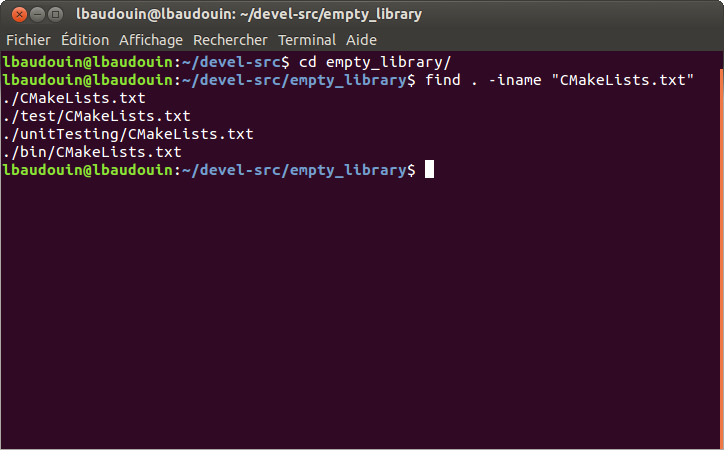
\includegraphics[width=\linewidth]{images/terminal-exemple}

\end{frame}

\subsection{Fonctions utiles}

\begin{frame}[fragile]{Fonctions utiles}
\begin{block}{Fonctions}
\begin{itemize}
\item \textbf{cd} : se déplacer d'un dossier à l'autre (., .., $\sim$, /, -)
\item \textbf{ls} : liste les fichiers (voir aussi \textbf{tree})
\item \textbf{mv,cp,rm} : déplace, copie, supprime des fichiers
\item \textbf{cat} : affiche le contenu d'un fichier (more, less, head, tail)
\item \textbf{grep} : cherche du texte dans un fichier
\item \textbf{find} : cherche un fichier suivant un pattern
\item \textbf{ssh} : se connecte à un serveur distant
\item \textbf{scp} : copie sur un serveur distant
%\item \textbf{locate} : cherche un fichier par son nom (updatedb)
\item \textbf{sed} : remplace du texte dans un fichier
\item \textbf{man} : affiche de l'aide
\end{itemize}
\end{block}
\end{frame}

\subsection{Utilisation}

\begin{frame}[fragile]{Aide}

\begin{block}{Paramètres}
\textcolor{cyan}{\verb?program [-v] [-o option] <input>?} \linebreak 
Options courantes pour l'aide : \verb?-h --help?
\end{block}

\begin{block}{Variables}
Définir une variable :
\textcolor{cyan}{\verb?myvar="data"?} \linebreak
Utilisation de la variable :
\textcolor{cyan}{\verb?\$myvar?} \linebreak

Variables prédéfinies : \textcolor{cyan}{\verb?\$HOME, \$USER, \$PWD, ...?}
\end{block}

\end{frame}


\subsection{Configuration de la console}

\begin{frame}[fragile]{Bashrc/Aliases}
\begin{block}{Bashrc}
\textcolor{cyan}{\verb?/home/\$USER/.bashrc ?} \linebreak
Fichier parsé au lancement d'une console, il permet de configurer la console (apparence, variable d'environnement, alias, \dots ).

Mise à jour : \verb?source ~/.bashrc?
\end{block}
\begin{block}{Aliases}
\textcolor{cyan}{\verb?/home/\$USER/.bash\_aliases ?} \linebreak 
Fichier parsé via le .bashrc\linebreak
Contient tout les alias et fonctions définit par l'utilisateur
Exemple: \verb?alias inst='sudo apt-get install '?
\end{block}
\end{frame}


\section{Système de fichiers}
\subsection{Système de fichiers}

\begin{frame}{Arborescence de Linux}
\begin{block}{File System}
\begin{tabular}{l l}
\textcolor{red}{/} & $\Leftarrow$ Racine\\
\textbar- \textcolor{red}{bin} & $\Leftarrow$ Binaires\\
\textbar- \textcolor{red}{home} & $\Leftarrow$ Utilisateurs\\
\textbar~\textbar- \textcolor{dgreen}{\$USER} & $\Leftarrow$ Utilisateur (raccourci : $\sim$)\\
\textbar~\textbar~\textbar- \textcolor{dgreen}{devel} & $\Leftarrow$ Dossier d'installation local (à créer)\\
\textbar~\textbar~\textbar- \textcolor{dgreen}{devel-src} & $\Leftarrow$ Dossier de sources (à créer)\\
\textbar- \textcolor{red}{lib} & $\Leftarrow$ Bibliothèques\\
\textbar- \textcolor{cyan}{usr} & $\Leftarrow$ User System Resource\\
\textbar~\textbar- \textcolor{cyan}{bin} & $\Leftarrow$ Binaires\\
\textbar~\textbar- \textcolor{cyan}{lib} & $\Leftarrow$ Bibliothèques\\
\textbar~\textbar~\textbar- \textcolor{cyan}{pkgconfig} & $\Leftarrow$ Fichiers de package\\
\textbar~\textbar- \textcolor{cyan}{share} & $\Leftarrow$ Données partagées
\end{tabular}
\end{block}
\end{frame}

\begin{frame}[fragile]{Installation locale}

\begin{block}{Créer les dossiers de travail}
\textcolor{cyan}{\verb?mkdir -p $\sim$/devel?}\linebreak
\textcolor{cyan}{\verb?mkdir -p $\sim$/devel-src?}
\end{block}

\begin{block}{A la fin du $\sim$/.bashrc}
\begin{scriptsize}
\begin{verbatim}
export LD_LIBRARY_PATH="${LD_LIBRARY_PATH}:${HOME}/devel/lib/"
export PKG_CONFIG_PATH="${PKG_CONFIG_PATH}:${HOME}/devel/lib/pkgconfig/"
export CMAKE_PREFIX_PATH="${CMAKE_PREFIX_PATH}:${HOME}/devel/share/"
export CMAKE_LIBRARY_PATH="${CMAKE_LIBRARY_PATH}:${HOME}/devel/share/"
export PATH="${PATH}:${HOME}/devel/:${HOME}/devel/bin/"
export CPATH="${CPATH}:${HOME}/devel/include/"
\end{verbatim}
\end{scriptsize}
\end{block}
\end{frame}

\section{Accès distant}

\subsection{}

\begin{frame}[fragile]{Connexion à distance}
\begin{block}{ssh}
\textcolor{cyan}{\verb?ssh [user@]<ip\_address>?} \linebreak
Exemple : \linebreak
\textcolor{cyan}{\verb?ssh devel@192.168.1.10?}
\end{block}

\begin{block}{Copie}
\textcolor{cyan}{\verb?scp [-r] <files> [user@]<ip\_address>:<path>?} \linebreak
Exemple : \linebreak
\textcolor{cyan}{\verb?scp image0.png devel@192.168.1.10:Images/?}
\end{block}
\end{frame}

\begin{frame}[fragile]{Connexion à distance}
\begin{block}{Configuration}
\textcolor{cyan}{\verb?cat .ssh/config?}
\begin{verbatim}
Host laptop
  HostName 192.168.1.100
  User leo
  Port 18000
\end{verbatim}
\end{block}

\begin{block}{Connexion rapide}
\textcolor{cyan}{\verb?ssh laptop?} 
\end{block}
\end{frame}


\section{Exemples}

\subsection{}

\begin{frame}[fragile]{Exemple}
\begin{block}{Navigation}
\begin{verbatim}
cd         #Retourner au dossier personnel
\end{verbatim}
\begin{verbatim}
cd module  #Entrer dans le dossier module
\end{verbatim}
\begin{verbatim}
cd ..      #Retourner au dossier parent
\end{verbatim}
\begin{verbatim}
cd -       #Retourner au dossier précédent
\end{verbatim}
\end{block}
\end{frame}



\begin{frame}[fragile]{Exemple}
\begin{block}{Recherche}
\begin{verbatim}
grep -sni "Text" *.cpp
\end{verbatim}
\begin{verbatim}
find . -name "get*.cpp"
\end{verbatim}
\begin{verbatim}
locate getText.cpp
\end{verbatim}
\end{block}
\end{frame}


\begin{frame}[fragile]{Exemple}
\begin{block}{Manipulation de fichier}
\begin{verbatim}
cat log.txt
\end{verbatim}
\begin{verbatim}
sed "s;un;deux;g" -i log.txt
\end{verbatim}
\begin{verbatim}
wc -w log.txt
\end{verbatim}
\end{block}
\end{frame}

\begin{frame}[fragile]{Exemple}
\begin{block}{Enchaîner des commandes}
\begin{verbatim}
cat list.txt | awk '{ print $2 }'
\end{verbatim}
\end{block}
\begin{block}{Lancer en arrière plan}
\begin{verbatim}
firefox https://gitlab.com &
\end{verbatim}
\end{block}
\end{frame}

\begin{frame}[fragile]{Exemple}
\begin{block}{Traduction}
\begin{verbatim}
function fren(){
  if test $# = 1; then
    firefox http://www.wordreference.com/fren/$1 &
  else
    firefox "http://translate.google.fr/#fr|en|$*" &
  fi
}
\end{verbatim}
\end{block}
\end{frame}

\begin{frame}[fragile]{Exemple complexe}
\begin{block}{finder.sh}
\begin{verbatim}
seq 1 150 | timeout 2 parallel -j 150 \
  bash -c 'echo > /dev/null && \
  exec 3<>/dev/tcp/192.168.1.{}/17000 && \
  r=$(cat <&3) && [ "$r" != "" ] && \
  echo "192.168.1.{} -> $r" && \
  exec 3>&- ' 2> /dev/null
\end{verbatim}
\end{block}
\end{frame}


%-------------------------------------------------------------------
\end{document} 

